\section{Inference Pipeline}
The app never trains a model. For every request, the backend takes a weather
forecast and turns it into hourly power for the user's rooftop. This section
describes that pipeline and the assumptions in it. The gradient boosting model
is used because it had the best test results.

\subsection{From Forecast Weather to Rooftop Power}
\begin{enumerate}
  \item The backend downloads the hourly forecast of shortwave radiation
        (W/m$^2$) and air temperature for the chosen city from the Open-Meteo
        forecast API, in Pakistan time.
  \item Irradiation is the radiation divided by 1000, because the Kaggle
        training data is in kW/m$^2$.
  \item No forecast gives the module temperature, so it is estimated as the
        air temperature plus $0.03125 \times$ the radiation in W/m$^2$ (the
        usual NOCT rule for a panel that reaches 45\,$^{\circ}$C).
  \item The hour and month are turned into sine and cosine values, and the
        three numeric inputs are scaled with the same \texttt{StandardScaler}
        that was fitted during training.
  \item The model needs an inverter ID as input, so it is run once for each
        of the 22 inverters and the predictions are averaged, which stands for
        a typical inverter.
  \item Each prediction is divided by the model's prediction for full sun
        (1 kW/m$^2$, 25\,$^{\circ}$C panel) at the same hour and month. This
        gives an output fraction between 0 and 1, which removes most of the
        scale of the Indian plant. The fraction is set to zero when there is
        no sunlight.
  \item The fraction is multiplied by the system size in kW and by a loss
        factor of 0.86 to get the power in kW for each hour.
  \item The hourly kW values are summed per day to get kWh per day, which is
        multiplied by the tariff to get the savings in rupees.
\end{enumerate}

\subsection{Assumptions}
\begin{itemize}
  \item \textbf{Loss factor of 0.86:} a common default for wiring, dust and
        inverter losses. It is an assumption, not a measured value.
  \item \textbf{Estimated module temperature:} the NOCT rule above, because
        forecasts do not include it.
  \item \textbf{Typical inverter:} the 22 inverter predictions are averaged.
  \item \textbf{Output fraction:} the plant's own size cancels out because the
        model is compared with its own full-sun prediction.
\end{itemize}

\subsection{Sample Predictions}
Figure~\ref{fig:samplepred} shows a 3-day forecast of a 5 kW system in each of
the five cities, with the model next to a simple physics baseline (sunlight
times system size, reduced by heat and the same loss factor). Both lines are
zero at night, rise in the morning and peak around midday. The gap between
the two lines shows how far the learned model differs from a fixed formula.
In these three days, Karachi achieves the highest output (around 20.8 to
21.0~kWh per day), while Peshawar has the lowest overall output (dropping to
12.3~kWh on the third day, with Lahore dipping to 11.4~kWh), and the learned
model consistently predicts slightly higher energy than the physics baseline.

\begin{figure}[H]
\centering
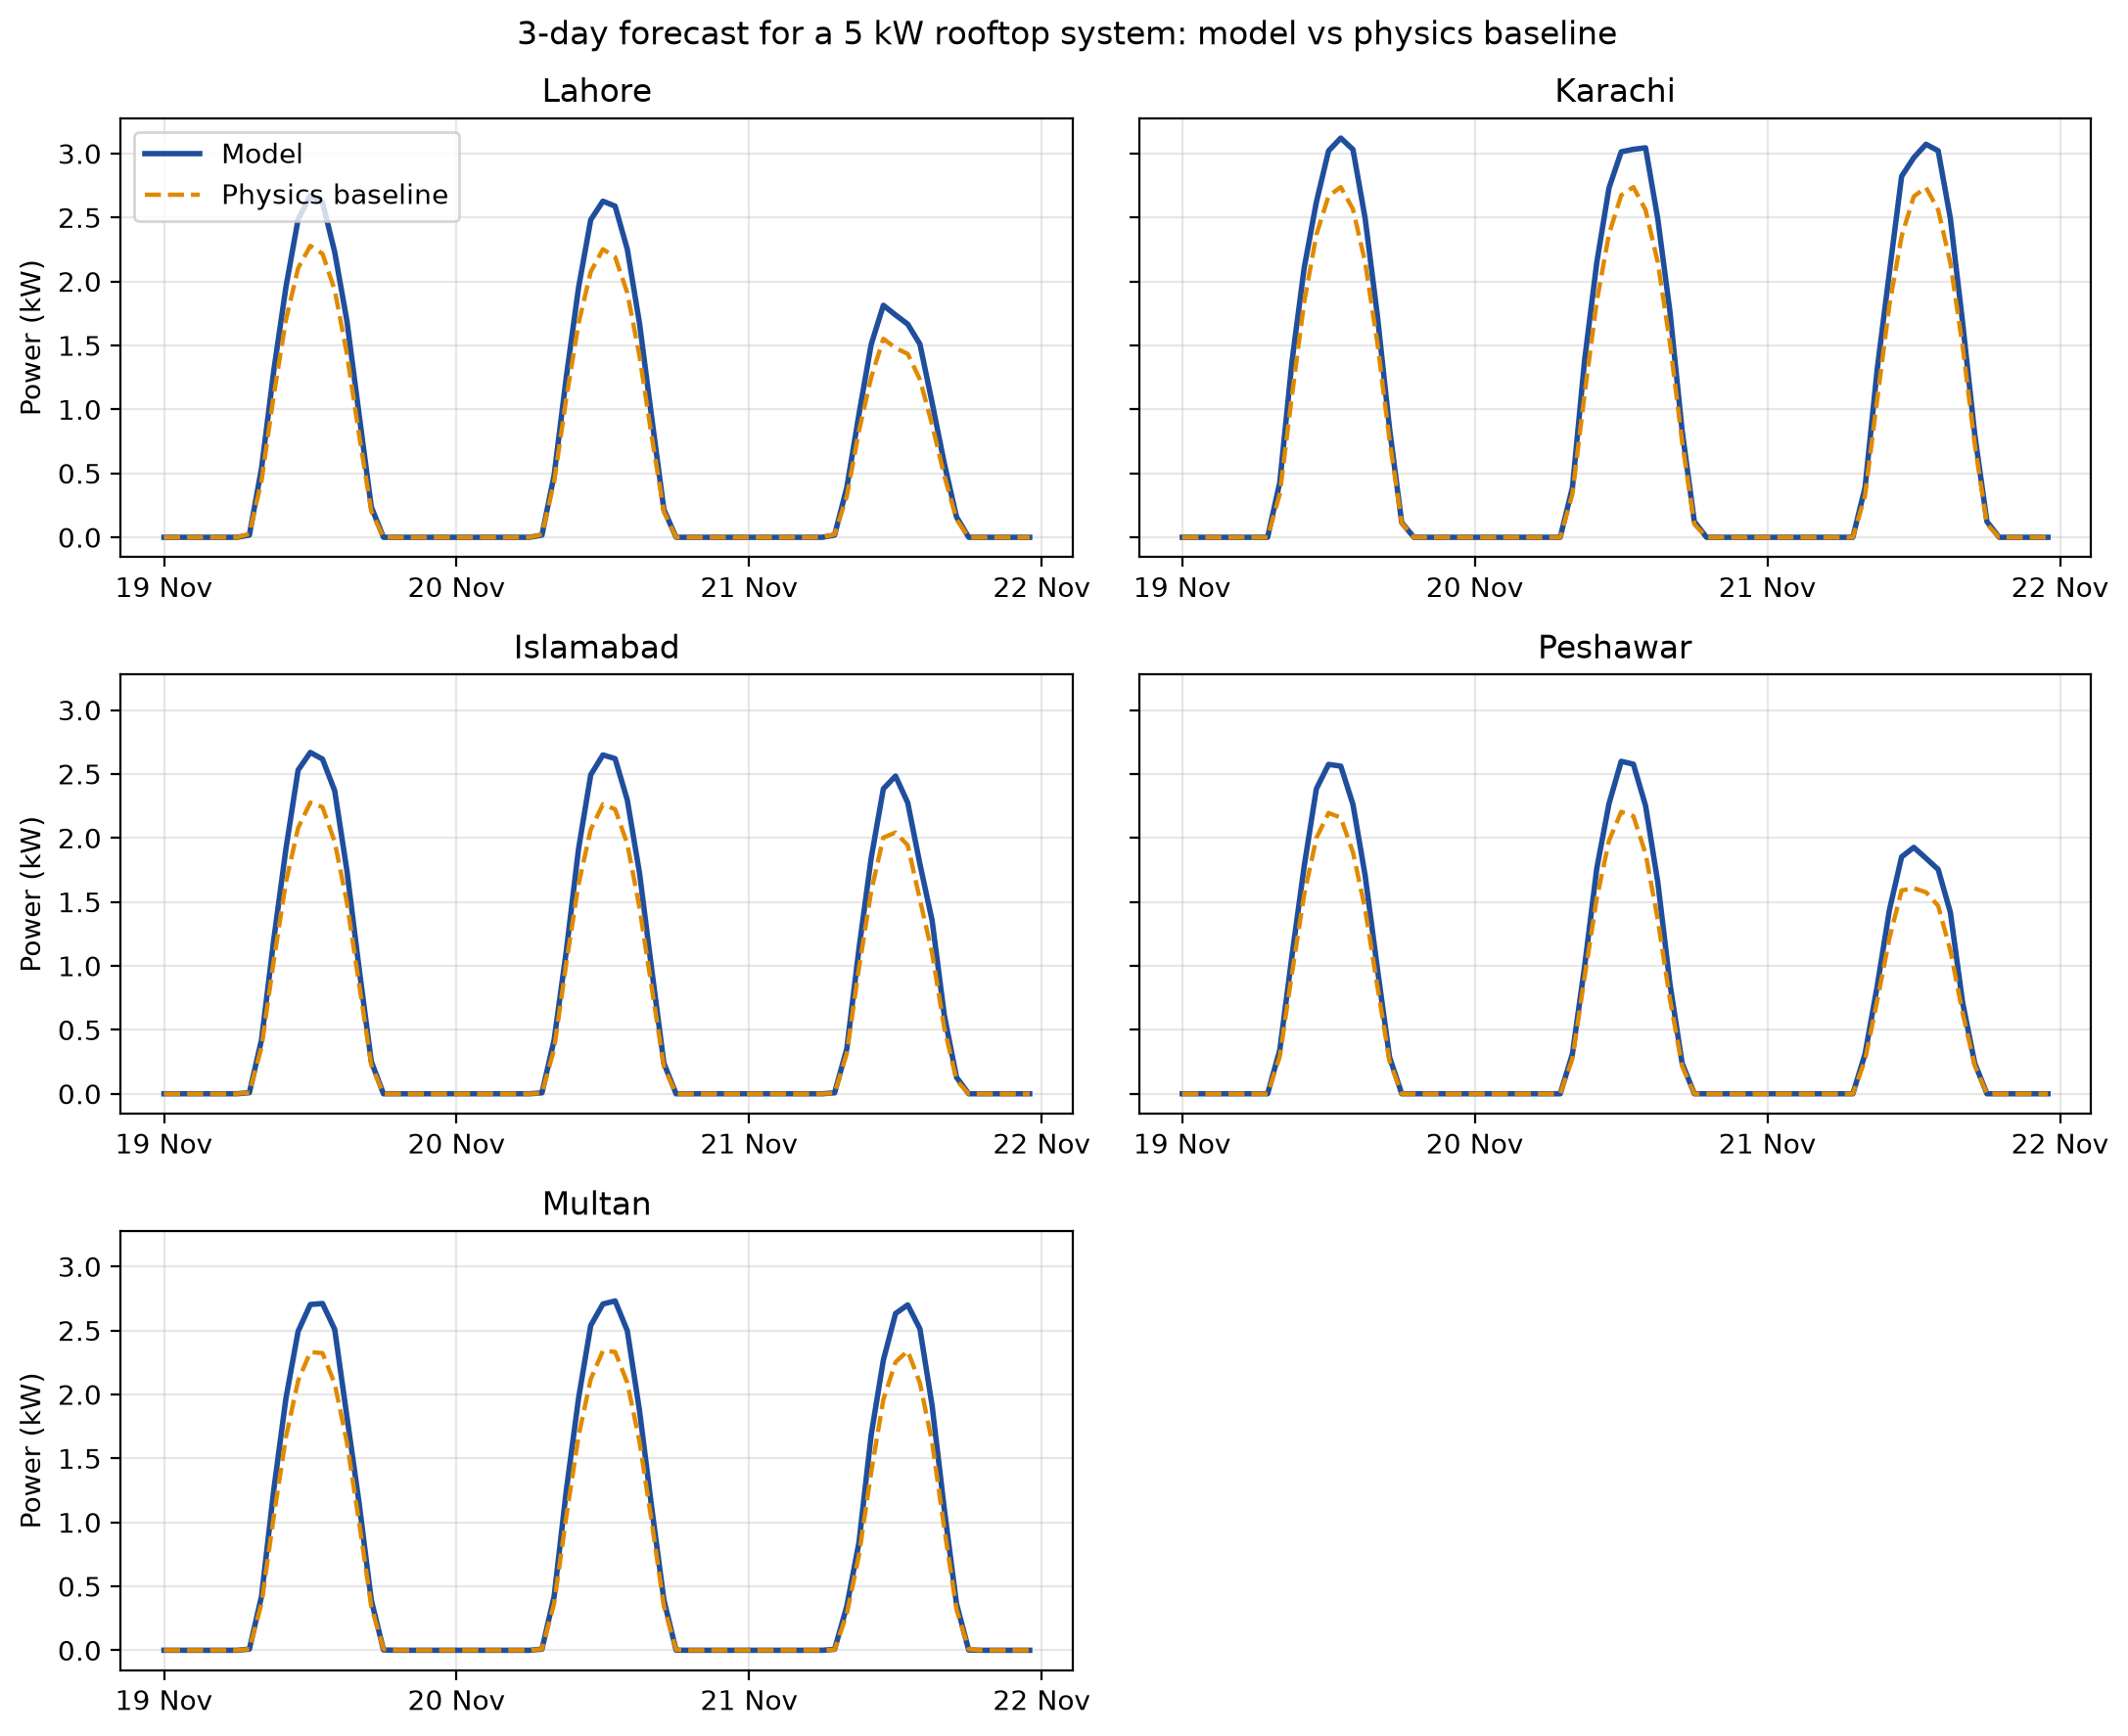
\includegraphics[width=\textwidth]{sample_predictions.png}
\caption{Three day forecast for a 5 kW rooftop system in five cities: model
versus physics baseline.}
\label{fig:samplepred}
\end{figure}

\subsection{Limitations of the Inference}
\begin{itemize}
  \item The model was trained on a single plant in India and only saw May and
        June, so winter and smog forecasts depend mostly on the radiation
        input.
  \item Errors in the forecast weather pass directly into the predicted
        output.
  \item The module temperature and the loss factor are estimates.
  \item The savings assume that all the energy is used by the household;
        surplus sent to the grid is paid at a lower rate.
\end{itemize}